\documentclass{standalone}

\usepackage{tikz}
    \usetikzlibrary{arrows.meta}

\usepackage{graphicx} % Работа с графикой \includegraphics{}
\graphicspath{{./images/img1/}} % картинки в папке ./images/img1/
    
\begin{document}

\begin{tikzpicture}
    % \draw[help lines] (-4,-3) grid (10,3);
    \node  at (0,0) 
        {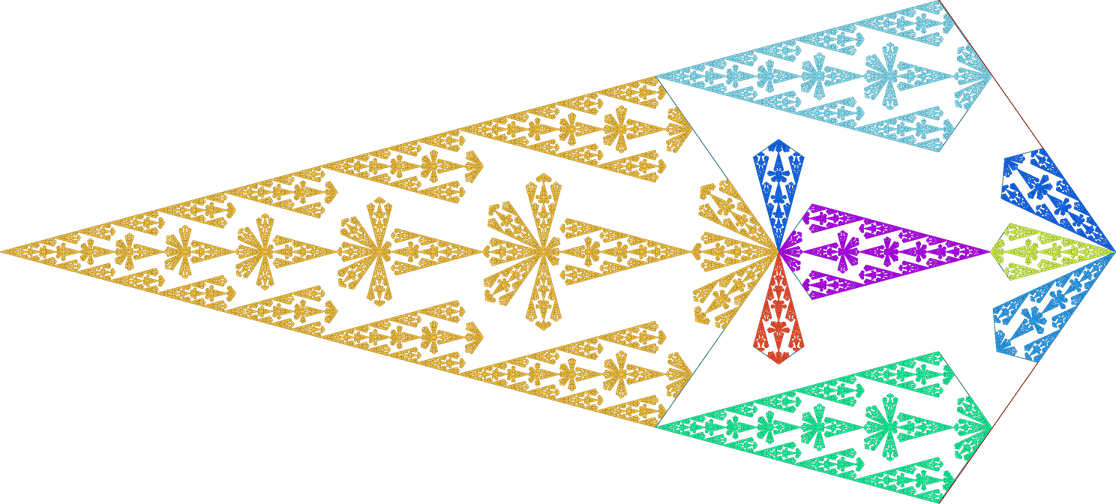
\includegraphics[width=85mm]{rpt6.png} };
    \node[shape=circle, draw, red, line width=1pt] 
        (k1) at (6,-1.5) {\large$1$};
    \node[shape=circle, draw, red, line width=1pt] 
        (k2) at (9,-1.5) {\large$2$};
    \node[shape=circle, draw, line width=1pt] 
        (k3) at (9,1.5) {\large$3$};
    \node[shape=circle, draw, red, line width=1pt] 
        (k4) at (6,1.5) {\large$4$};
    \path[->, >={Latex[length=7pt]}, line width=1pt] 
        (k1) edge[loop left, distance=1cm, red] node[shift={(0.6,0.4)}, black]{$1$} (k1)
        (k2) edge[loop left, distance=1cm, red] node[shift={(0.6,0.4)}, black]{$3$} (k2)
        (k4) edge[loop left, distance=1cm, red] node[shift={(0.6,0.4)}, black]{$2$} (k4)
        (k3) edge[bend left=30] node[above]{7}(k1) 
             edge[thick, bend right=30] node[above]{9} (k1) 
             edge node[above]{8} (k1);
    \fill[black] (-4.2,0)
         circle (0.07) 
         node[left=1mm]  {\large$1$};
    \fill[black] (2.9,-1.95) 
         circle (0.07) 
         node[below=1mm] {\large$2$};
    \fill[black] (4.25,0)
         circle (0.07) 
         node[right=1mm] {\large$3$};
    \fill[black] (2.9,1.95) 
         circle (0.07) 
         node[above=1mm] {\large$4$};
    \node at (-1,1.2){{$P_1$}};
    \node at (2,2){ $P_2$};
    \node at (2,-2){ $P_3$};
    % \node at (2.7,0.3){$P_4$};
    % \node at (2.1,0.7){$P_5$};
    % \node at (2.1,-0.7){$P_6$};
    \node at (3.6,0){$P_7$};
    \node at (4.1,0.6){$P_8$};
    \node at (4.1,-0.6){$P_9$};
\end{tikzpicture}

\end{document}